\documentclass[letterpaper]{article}
\usepackage{graphicx}
\usepackage{fullpage}
\usepackage{color}
\usepackage[english]{babel}
\usepackage{appendix}
\usepackage{tabularx}


\newcommand{\HRule}{\rule{5cm}{0.1mm}}
\begin{document}
\begin{center}


% Upper part of the page
%
\includegraphics[\textwidth]{SSDDTemplateA2-img1}\\[1cm]    

\textsc{\Large University of Idaho}\\[0.2cm]

\textsc{\Large CS481: Senior Design}\\[2cm]


% Title
{ \LARGE \bfseries Idaho Department of Health and Welfare}\\[0.4cm]
{ \huge \bfseries Time, Accounting, and Reporting System}\\[1.0cm]
{ \normalsize \emph{ prepared for}}\\[0.5cm]
{ \normalsize Don Moreaux}\\[0.5cm]
\HRule \\[3cm]

% Authors and supervisors
\begin{minipage}{0.4\textwidth}
\begin{flushleft} \large
\emph{Authors:}\\
Scott Beddall\\
Brett Hitchcock\\
Chaylo Laurino\\
Alex Nilson
\end{flushleft}
\end{minipage}
\begin{minipage}{0.4\textwidth}
\begin{flushright} \large
\emph{Advisors:} \\
Greg Donohoe\\
\bigskip
\bigskip
\bigskip
\bigskip
\end{flushright}
\end{minipage}

% Bottom of the page
{\large \today}

\end{center}
\pagebreak


\pagebreak
\section{\bfseries{Introduction}}
\subsection{\bfseries{Identification}}
This Software Design Document pertains to the Idaho Department of Health and Welfare Time, Accounting, and Reporting System. Project development for Fall Semester, 2011 is executed by Scott Beddall, Brett Hitchcock, Chaylo Laurino, and Alex Nilson. The advisor for the project from the University of Idaho is Gregory Donohoe. Our project sponsor and primary client from the Idaho Department of Health and Welfare is Don Moroeux. 
\subsection{\bfseries{Document Purpose, Scope, and Intended Audience}}
\subsubsection{Document Purpose}
This document's sole purpose is to outline the scope of Idaho TARS. This outline includes, but is not limited to:
\begin{itemize}
\item Development decisions and their reasoning.
\item Architectural Specifications.
\item Detailed Design Information.
\item Locations of Other Project Resources.
\end{itemize}
\subsubsection{Document Scope and/or Context}


\subsubsection{Intended Audience for Document}
Though the TARS is to be fully prototyped by the end of 2011, it will not be completed. With that being the case, this document is aimed at any future developers or users of Idaho TARS. 

\subsection{\bfseries{Software Purpose, Scope, and Intended Users}}
\subsubsection{Software Purpose}
Idaho TARS is intended to provide time and resource tracking for contractor/non-contractor work efforts within the Idaho Department of Welfare. Work efforts must be added to time-bounded project PCA codes and approved by users with sufficient privileges. Project summaries, cost totals, and other information will then be available within the TARS.     

\subsubsection{Software Scope/Context}
The Idaho Department of Health and Welfare currently is utilizing a resource called Mariner for project management. The IDHW's needs, however, are significantly less than the capabilities that Mariner provides. Portfolio and Resource Management, Planning, and other features of Mariner are being paid for, but being left unused. This is where the creation of the Time, Accounting, and Reporting System is merited. 

\subsubsection{Intended Users for the Software}
Intended Users of Idaho TARS are the staff and employees of the Idaho Department of Health and Welfare as well as their contractors.

\subsection{\bfseries{Definitions, Acronyms, and Abbreviations}}
A Table should go here. 

\subsection{\bfseries{Document Overview}}
Section 2 describes software constraints imposed by the operation environment, system requirements, and user characteristics. After this it will identify the system stakeholders and list/describe their concerns.  \\
\\
Section 3 of this document describes the system and software
architecture from several viewpoints, including, but not limited to,
the developer{\textquoteright}s view and the user{\textquoteright}s
view.\\
\\
Section 4 provides detailed design descriptions for every component
defined in the architectural view(s). \\
\\
Sections 5 provides traceability information connecting the original specifications
(referenced above) to the architectural components and design entities identified in this document.\\
\\
Section 6 and beyond are appendices including original information and communications used to create this document.
\section{\bfseries{Software Requirements, Constraints, and User Characteristics}}
%\subsection{Software Requirements}

\subsubsection{PCA Requirements}

\bf{PCA-1} \\
Users with the proper permissions must be able to manually enter PCA codes in a form that meets DHW standards.\\
\paragraph{}
This provides the ability to correctly connect the PCA code(s) to work, and ensures we are correctly accounting for what costs are allocated to what work. Work can be project related, a maintenance activity, or a non-productive activity such as meeting time.\\
Status:\bfseries{In Progress}\\

\bfseries{PCA-2}\\
\paragraph{}
Users with proper permissions must be able to manually tie work effort(s) to valid PCA.\\
Description\\
Status:\bfseries{ In Progress}\\

The system must provide a mechanism for time bounding PCA codes - with the ability to "deactivate" a code prematurely and an open "end" date.\\

Must maintain an audit trail (history of changes - people, projects, and PCAs).

The system must provide a mechanism for preventing time to be allocated to expired PCA codes.

The system must allow multiple PCA to be assigned to a work effort, over the life of the effort/project.

Must be able to assign one or more PCA codes to work effort (split percent allocation across multiple PCAs which can change during life of work effort)

Must allow work to be assigned to other entities outside DHW

Must allow work to be associated with multiple divisions or the enterprise.

\subsubsection{Data Requirements}
The system shall track date specific vendor and employee/contractor information

The system shall allow for some description of work or project to be entered and attached.

The system shall be consistent with I-Time data

The system shall provide a means to replicate last week's assignments (repeating tasks can auto fill)

The system must have a method that allows staff to create work effort, and self-assign

Must be able to track work effort for resources, depending upon their assignment, that are either cost allocated or not cost allocated.

Must be able to break time out by time codes for work efforts, such as Vacation, Sick, LWOP, (match I-Time data since this is the system of record)

Users shall have the ability to close tasks and activities on their timesheet, and reopen if needed.

The system shall provide some mechanism (configurable dropdown) for  grouping of business, program, and function of work.

Audit trail data shall include the information that was updated, modified/deleted, date created, and by whom for each item determined to be auditable.

Data for staff and projects shall include the ability to store links and attachments

The system must allow for future time entry

Must prevent work efforts to exist in the system unless they are tied to a PCA code.

All data for reporting shall be extracted via external source (EDW. Excel, etc.).

Must allow users to create a view of their I-Time timesheet. 

Reports must be real-time, reliable, and accurate. Includes exports to csv, Excel. 

Must have a sort and group function that allows work effort to be grouped by application, division, manager, etc.

The system must allow a user the ability to create a custom view of the data.

Must allow users to easily size windows.

Must be able to limit view of information presented to user to what is pertinant to that user's role.

The system shall provide search/find functionality to locate work efforts, with minimal amount of navigation (task actions less than clicks/pages/dialogs)

Must authenticate to Active Directory

Must have a role-based permissions security.

The system shall allow for automated closure of time periods for PCA and work efforts, with administrator ability to manually reopen and close for edit and approval.

The system must allow each user the ability to navigate easily by logic/functional areas, ie. Staff demographics, projects, work items/areas, time entry, etc.

Must automatically display current week when entering timesheet data.

Must have notifications (via email, context) triggered by certain events such as timesheet submittal, approvals, PCA expiration. 

Users with permissions, must have the abiltiy to approve TARS weekly submittals.

\section{Software Architecture}
\subsection{Server Architecture - Microsoft Internet Information Services 7} 
Microsoft's Internet Information Services server is a modular, intuitive server application. Since the IDHW uses Windows Server for most of their infrastructure, Idaho TARS will do the same. New considerations must now be applied, however. IIS7, being a Microsoft product, uses Microsoft development software. Namely:
\begin{itemize}
\item C\# 
\item ASP.NET
\item Visual Basic/VB.NET
\item .NET Development Framework
\end{itemize} 
TARS will be developed using all these technologies, as well as the IIS7 MVC application. The MVC application will be described in detail in the next section.

\subsection{Model-View-Controller}
Most of the heavy-lifting for TARS will be present in the display and interaction with large amounts of data. This problem is what the Model-View-Controller design pattern was created for. The idea is that each word in the acronym: Model, View, and Controller each handle a different aspect of the display process.
\subsubsection{Controller}

\subsubsection{Model}

\subsubsection{View}

\subsection{MySQL Database}
Since TARS is being developed for IIS7, our databases will be in MySQL format. Any queries made by the MVC will be carried out by the \"Model\" controller. 

\subsection{Active Directory}
The IDHW uses Microsoft Active Directory for their user authentification. With that infrastructure already in place, it is logical to use the same for Idaho TARS. 

\subsection{Security}
While Idaho TARS will be used internally, there is still a security risk. The system may not be dealing with any highly confidential info, but TARS will have access to government resources like the IDHW Active Directory and I-Time interfaces. To prevent easy exploitation of the TARS databases, all queries to the database will be centralized in Model. This will will not only make the team's code more readable, but also make it more secure. Centralized queries allow us to easily implement a strong security stance. Namely, all input from anywhere on the browser will be treated as \"tainted.\" This tainted input will not be used for any queries on the MySQL database until it has been cleansed.


\subsection{Browser Interface}
Though it is probably already indicated by the server architecture, the development team must make it clear that this software is being developed for a web interface. This will eliminate many of the dependencies that are inherent to a system launched from a binary. The development team is developing this project to meet the following end system requirements:
\begin{itemize}
\item 1024x768 monitor resolution
\item Google Chrome
\item Mozilla Firefox
\item Internet Explorer 7 and up
\item Safari
\end{itemize}
\section{Design Descriptions}
\subsection{Model-View-Controller Modules}
To be filled in as classes are stubbed out.
\subsection{MySQL Database Schema and Interface Description}
As mentioned above in the Software Architecture section, TARS will use a MySQL database to store all interactions other than User Info. Before outlining the Database Schema, it would be wise to fully describe the thought process of the development team.\\
\\
Stripped down to its most base parts, TARS is simply a database interface through which users can log and retrieve hours to and from work efforts. These \"Work Efforts\" are simply general projects that can have hours of contractor/non-contractor work added to their totals. For instance, there might be a Work Effort that is assigned its own unique ID and whos description is \"Document the latest changes to the TARS SDD.\" Any employees who wish to log their hours will find the Work Effort's ID, add their hours along with other relevant data, and submit their entire worksheet for approval. \\
\\
The Work Effort to \"Document the latest changes to the TARS SDD.\" now has hours logged on it and waiting for approval. A user with the correct Active Directory permissions can now go check the status of the Work Effort, and approve any pending hours waiting on it. The development team has chosen to add all hours, approved or not, to the Work Effort's database table. A simple boolean present as a column in the table will ensure that filtering by approved/unapprooved will be a simple task.\\
\\
Unfortunately, the process is not done. Now that a Work Effort has hours charged to it, how can the accounting department charge these expenses? The simple answer is, they can't yet. To provide that functionality, PCA Codes must be assigned. This introduces another database table, as one PCA Code may have multiple Work Effort associations; just as one Work Effort may be associated with multiple PCA Codes.\\
\\
One final note about the Work Efforts and PCA Codes is needed. The requirements state that they both must be time-bounded, capable of early expiration, and renewable. \\
\\
Through discussion of the above situations and processes, the development team settled on the following database schema. These are no final by any means, as rarely does a design get finalized before development has commenced.\\
\\
\subsubsection{TARS Database Schema}
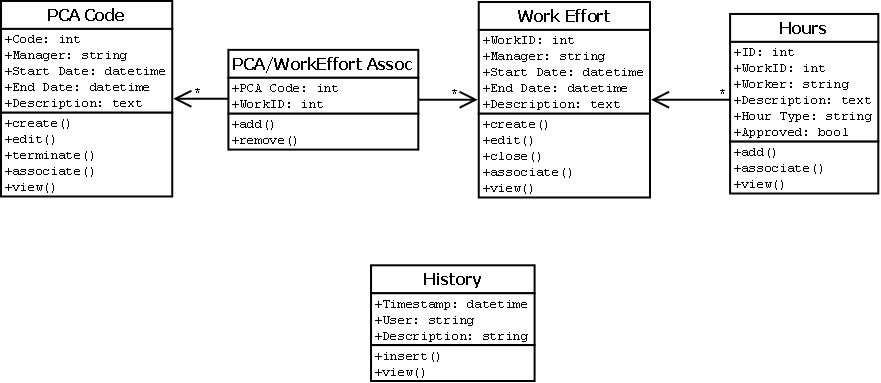
\includegraphics[scale=0.4]{../design/images/class_diagram_1.png}
\section{Tracability Information}
All effort on the project may be tracked via the project GitHub repository: github.com/ICBM/TARS\\
\\
Client requirements changes will be handled via email. Current progress on requirements as well as the requirements changelog is available at: https://github.com/ICBM/TARS/blob/master/doc/requirements\_summary.docx
\section{Appendix A: Use Cases} 
More might be required here.

\paragraph{Login}
\begin{enumerate}
\item Click the "Login" button
\item Enter username and password
\item Hit Enter or click "Submit"
\item System authenticates and redirects to home page.
\end{enumerate}

\paragraph{Adding new PCA code.}
\begin{enumerate}
\item Select "Add PCA"
\item System loads PCA form
\item Fill in form, including time bounds for the PCA code
\item Press "Submit"
\item System updates tables and redirects to new PCA display page
\end{enumerate}

\paragraph{Deactivating PCA code}
\begin{enumerate}
\item Select desired PCA code
\item System loads PCA display page
\item Click deactivate
\item Confirm deactivation.
\item System updates tables and locks PCA code.
\end{enumerate}

\paragraph{Adding Work Effort}
\begin{enumerate}
\item Select "Add Work Effort"
\item System loads Work Effort form
\item Fill in form
\item Associate desired PCA code or codes, if multiple PCA codes are chosen a percentage of work effort may be set for each
\item Associate entity or entities
\item Click "Submit"
\item System updates tables and redirects
\end{enumerate}

\paragraph{Add Employee/Contactor Info}
\begin{enumerate}
\item Select "Add Employee/Contractor"
\item System Loads Add Entity form
\item Fill in data
\item Click Submit
\item System Updates table and redirects
\end{enumerate}

\paragraph{Edit/Update Employee/Contractor Data}
\begin{enumerate}
\item Select desired entity
\item System pulls data from database and loads Entity Form
\item Edit/Update as desired
\item Click "Update"
\item System updates table and redirects.
\end{enumerate}

\paragraph{The system must allow for future time entry}
\begin{enumerate}
\item Select ``Add Work Effort''
\item Fill in form, making sure to add the effort to the correct date.
\item Click ``Submit''
\end{enumerate}

\paragraph{All data for reporting shall be extracted via external source (EDW. Excel, etc.).}
\begin{enumerate}
\item Under a given PCA code or work effort, select ``Get Data Report''.
\item The system will then generate a copy of the data in EDW or Excel format.
\item User saves the copy at a destination of their choosing.
\end{enumerate}

\paragraph{Must allow users to create a view of their I-Time timesheet.}
\begin{enumerate}
\item User logs in.
\item On the user's personal page, select ``Get I-Time Report''.
\item The system will then generate a copy of the data for viewing.
\end{enumerate}

\paragraph{Must have a sort and group function that allows work effort to be grouped by application, division, manager, etc.}
\begin{enumerate}
\item User logs in.
\item User selects ``My Work Efforts''
\item System generates list of all work efforts related.
\item User selects to sort by name, application, etc.
\item System sorts and redisplays work efforts in the proper order.
\end{enumerate}

\paragraph{The system must allow a user the ability to create a custom view of the data.}
\begin{enumerate}
\item User selects a PCA code or Work Effort code
\item User selects ``Get Data Report''.
\item User enters custom settings and hits ``Select''.
\item System generates report.
\end{enumerate}

\paragraph{Must allow users to easily size windows}
\begin{enumerate}
\item User resizes browser, which will resize the web interface.
\end{enumerate}

\paragraph{The system shall provide search/find functionality to locate work efforts, with minimal amount of navigation (task actions<=4 clicks/pages/dialogs)}
\begin{enumerate}
\item User logs in.
\item User navigates to a work effort by...
\begin{itemize}
  \item Clicking on a link in the ``My Recent Work'' bar.
  \item Entering a Work Effort code or PCA code in the Search bar on the top.
    \end{itemize}
\end{enumerate}

\end{document} 
